\chapter[Processo da Engenharia de Requisitos]{Processo da Engenharia de Requisitos}
O processo descrito a seguir foi modelado na ferramenta Bizagi BPMN Modeler. Esta ferramenta foi escolhida após uma comparação com a ferramenta Bonita BPM, levando em conta critérios como popularidade, acessibilidade e funcionalidades disponíveis para o desenvolvimento do projeto.

Como dito anteriormente a abordagem a ser utilizada será uma abordagem ágil, fundamentada no SAFe (Scaled Agile Framework), utilizando os três níveis principais: Portfolio, Programa e Time. O nível de Fluxo de Valor não será utilizado por se entender que não há necessidade deste nível neste projeto.

A estrutura dos três níveis do SAFe foi mantida porque, segundo Leffingwell (2011), ao diminuir nível de abstração dos requisitos gradativamente, diminui também o nível de especificação precoce, reduzindo a sobrecarga ao gerenciar os requisitos. Isso também aumenta a agilidade do time por permitir a interpretação dos requisitos de maneira mais fácil para a implementação.

A gestão da rastreabilidade dos requisitos é de suma importância para a manutenção desse processo. Todavia, o SAFe não define consistentemente a manutenibilidade entre seus três níveis, refletindo em uma escolha da equipe por adotar atividades de gerência de mudanças do RUP. Essa abordagem é explicada na Seção [SEÇÃO]. É importante dizer que o SAFe considera sim a mutabilidade dos requisitos e que essa escolha é uma maneira encontrada para lidar com essas mudanças e seus respectivos riscos da melhor forma possível.

Um fator determinante para a aplicabilidade do SAFe a uma equipe mínima e um projeto de pequeno porte, é a consistência na seleção dos papeis que vão compor o processo. De acordo com a análise da viabilidade de tempo e recursos, do problema proposto e do cliente, foram estabelecidos os seguintes papéis:

\begin{description}
\item[Especialista do Negócio] É o stakeholder que detém o conhecimento do negócio, do contexto organizacional e da visão do produto.    
\item[Product Owner (P.O.)] É o membro do time que fica responsável pela definição das histórias e pela priorização do Team Backlog, além de participar do planejamento e validação da sprint definindo os seus objetivos.
\item[Product Manager (P.M.)] De acordo com Leffingwell(2011), cabe ao P.M.: manter a visão e o program backlog, priorizar features, manter o roadmap, gerenciar o conteúdo da release e manter e priorizar o porfolio backlog. As atividades realizadas pelo P.M. acontecem nos níveis Portfolio e Program.
\item[Scrum Master] Seu papel é dar assistência para o resto da equipe a fim de extrair a máxima perfomance, ele é de certa forma o líder do time(Leffingwell, 2011).
\item[Time] É composto por toda a equipe, desenvolvedores, designers e etc.
\end{description}

\section{Big picture do processo}
  \begin{figure}[!htbp]
    \centering
    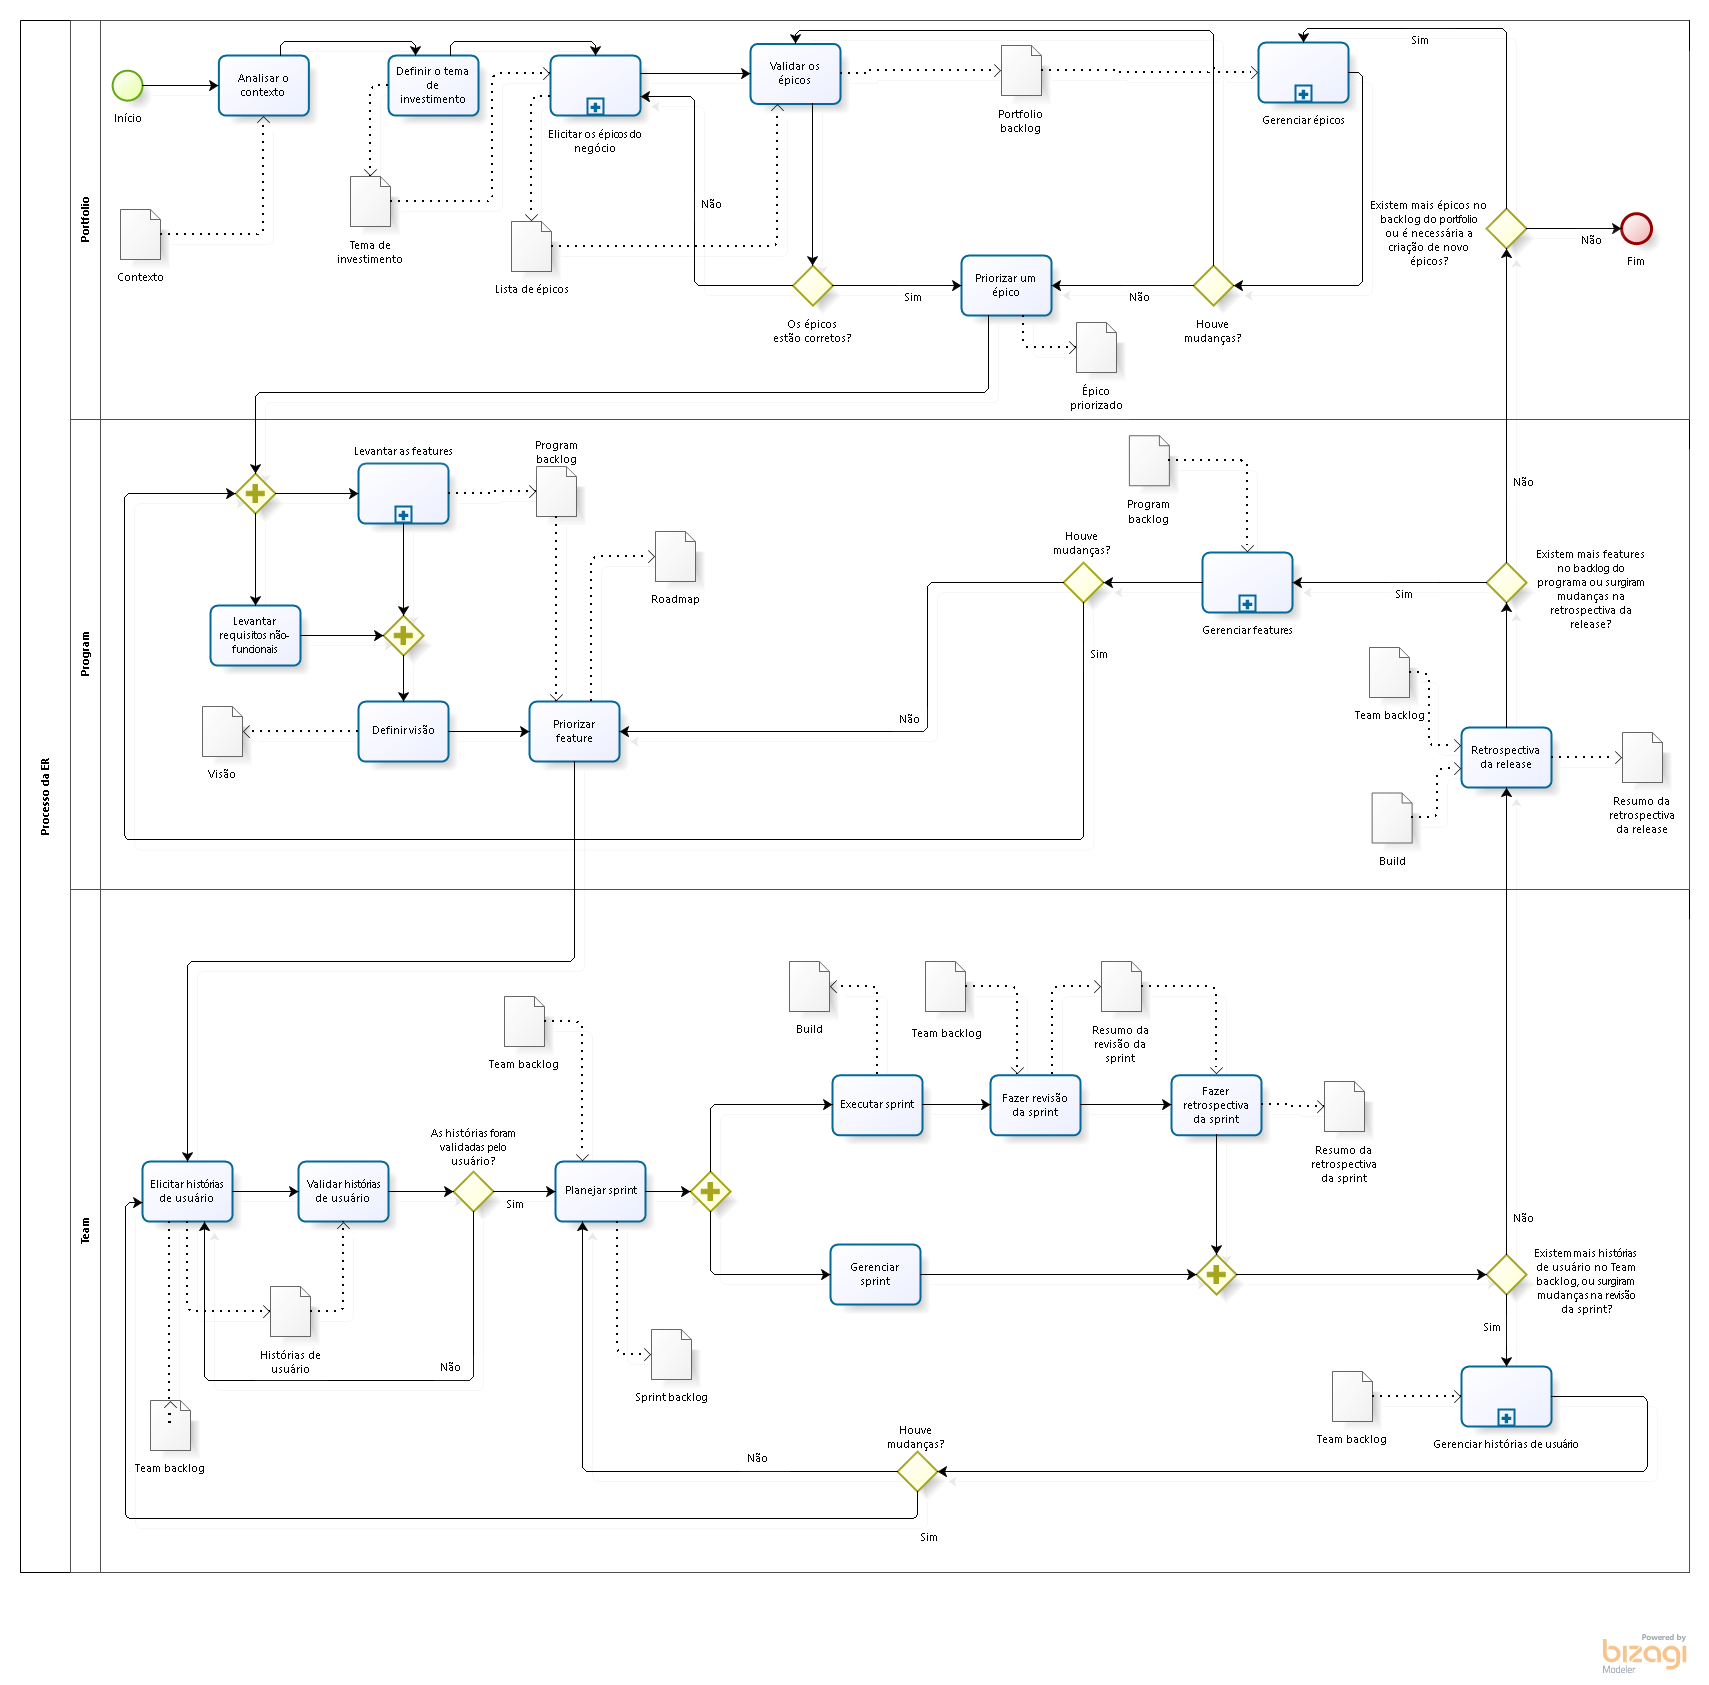
\includegraphics[scale=0.3]{figuras/Processo_v1-2}
    \caption[Big picture do processo.]{Big picture do processo. \footnotemark}
    \label{processo}
  \end{figure}

\section{Portfólio}
Esse nível tem como objetivo principal levantar e elaborar uma abstração de alto nível dos requisitos de negócio. Cada uma das atividades, artefatos gerados e papeis estabelecidos que serão descritos a seguir fazem parte da solução proposta para se resolver o problema existente. A execução de cada atividade será baseada na sistematização da análise documental e brainstorms.

\subsection{Artefatos}
\begin{description}
\item[Contexto do cliente] É fornecido pelo cliente ou levantado a partir de outras fontes de informação que contenham dados sobre o próprio cliente e o problema a ser resolvido. Este artefato descreve resumidamente uma visão do contexto do problema e do cliente.
\item[Tema de investimento] Consiste na documentação de quais são os reais objetivos e valores da empresa e os benefícios que a solução em software trará para a mesma. Por se tratar de um requisito de altíssimo nível é representado por uma breve descrição.
\item[Lista de Épicos] São iniciativas, ou frentes de negócio que podem gerar alto valor para o cliente, equipe ou o desenvolvimento de software em si, como inovações arquiteturais ou implementação de tecnologias emergentes. Por se tratar de um requisito de alto nível, precisa ser trabalhado e refinado.
  \begin{enumerate}
    \item \textbf{Tempo:} um épico pode demandar tempo e vários ciclos de iteração para ser devidamente implementado.
    \item \textbf{Escopo:} por ser de alto nível afeta os subsequentes níveis do projeto, ocasionando um grande impacto e sendo uma área crítica pode custar muito para a equipe/cliente.
    \item \textbf{Negócio:} Representa a entrega de valor direta para o cliente, afetando diversos departamentos da área de negócios.
  \end{enumerate} 
\item[Backlog do Portfólio] Contém o detalhamento de cada um dos épicos e devidamente priorizados e organizados. Para isso, a cada épico é atribuida uma pontuação de acordo com sua complexidade seu valor gerado. Logicamente, para realizar uma avaliação precisa da complexidade da implementação do épico é necessário um detalhamento do mesmo.
\end{description}

\subsection{Descrição das atividades}

\section{Programa}
Nessa etapa do processo se baseia na identificação de features e requisitos não funcionais, na elaboração das correspondentes histórias de usuário e no planejamento das entregas do software. Há também uma preocupação em se estabelecer estratégias para o desenvolvimento eficaz do software.

\subsection{Artefatos}
\begin{description}
\item[Program Backlog] É o documento onde as features são registradas, como uma pilha de features.
\item[Roadmap] Consiste em uma série de releases com datas planejadas, cada uma pertinente a um tema, um conjunto de objetivos e a priorização das features. O roadmap nos dá uma ideia de como a equipe planeja mostrar valor no decorrer do tempo (Leffingwell, 2011).
\item[Visão] É um mecanismo utilizado para definir e comunicar diversos aspectos do sistema. Segundo Leffingwell [2011] A visão de um sistema é composta por um conjunto de características que irão descrever as possibilidades do sistema, isto é, tudo aquilo que ele poderá oferecer ao usuário a fim de atender as necessidades dos envolvidos.
\end{description}

\subsection{Descrição das atividades}

\section{Time}
O nível da equipe descreve como as equipes ágeis aplicam o SAFe integrado com as práticas Scrum/XP e análise de qualidade para garantir a entrega da solução descrita nos documentos de requisitos.

\subsection{Artefatos}
\begin{description}
\item[Team Backlog] Representa uma coleção de tudo que o time necessita para implementar aquela parte do sistema. Pode conter histórias de usuário ou enabler histories. Sendo que a maioria tem origem no program backlog, enquanto algumas são pertinentes a um contexto específico do time. O team backlog pertence ao P.O., vale salientar que o fato de "pertencer" ao P.O. não significa que ele é o único que pode alterá-lo, mas é preferível que seja ele a fazer isso.(SAFe, 2015)
\item[Sprint Backlog] É uma lista de tarefas que o time se compromete a fazer em uma Sprint. Os itens do Sprint Backlog são extraídos do Team Backlog, com base nas prioridades previamente definidas. É a percepção da equipe sobre o tempo que será necessário para completar um conjunto de funcionalidades.
\item[Build] É o incremento gerado a cada sprint.
\end{description}

\subsection{Descrição das atividades}

\section{Artefatos}
\textbf{Temas de investimento} - Representam um conjunto de iniciativas guias para o investimento da instituição, seja em sistemas, produtos, aplicações ou serviços(Leffingwell, 2011).

\textbf{Épicos} - São iniciativas de desenvolvimento em larga escala que agregam valor a um tema de investimento(Leffingwell, 2011). São os de requisitos que possuem o mais alto nível no processo(Leffingwell, 2011).

\textbf{Portfolio backlog} - É o local onde os épicos são registrados, como um repositório de épicos.

\textbf{Features} - Atuam como pontes entre as necessidades dos stakeholders e os requisitos específicos no domínio da solução(Leffingwell, 2011).

\textbf{Program backlog} - É o local onde as features são registradas, como um repositório de features.

\textbf{Roadmap} - Consiste em uma série de releases com datas planejadas, cada uma pertinente a um tema, um conjunto de objetivos e uma feature priorizada. O roadmap nos dá uma ideia de como a instituição planeja mostrar valor com o decorrer do tempo(Leffingwell, 2011).

\textbf{Visão} - É um mecanismo utilizado para definir e comunicar a visão do sistema(Leffingwell, 2011). A visão de um sistema é composta por um conjunto de features que irão descrever as possibilidades do sistema, isto é, tudo aquilo que ele poderá oferecer ao usuário a fim de atender as necessidades dos envolvidos(Leffingwell, 2011).

\textbf{Team backlog} - Representa uma coleção de tudo que o time necessita para progredir aquela porção do sistema. Pode conter histórias de usuário ou enabler histories. Sendo que a maioria tem origem no program backlog, enquanto algumas são pertinentes a um contexto específico do time. O team backlog pertence ao PO, vale salientar que o fato de "pertencer" ao PO não significa que ele é o único que pode alterá-lo, mas é preferível que seja ele a fazer isso. (SAFe, 2015)

\textbf{Sprint backlog} - É o local onde serão armazenadas as histórias de usuário a serem realizadas naquela sprint.

\textbf{Build} - É o incremento de software gerado em cada sprint.

\section{Atividades}
